\documentclass{homework}
% \usepackage{graphicx} % Required for inserting images
\usepackage{amsmath}
\usepackage{gensymb}
\usepackage{subfig}
\usepackage{float}
\usepackage{pythonhighlight}



\class{APPM 5600}
\title{Homework 1}
\author{Sean Jennings}
\date{September 6, 2024}



% Python style for highlighting
\lstset{
language=Python,
basicstyle=\ttm,
morekeywords={self},              % Add keywords here
keywordstyle=\ttb\color{deepblue},
emph={MyClass,__init__},          % Custom highlighting
emphstyle=\ttb\color{deepred},    % Custom highlighting style
stringstyle=\color{deepgreen},
frame=tb,                         % Any extra options here
showstringspaces=false
}

\begin{document}
\maketitle

\section{Problem 1}
\begin{letterenum}
\item Let $f(x) = \sqrt(x + 1) - 1$. When $x$ is less than machine precision $\epsilon$, then
float$(1 + x) = x$, where float indicates the evaluation of the floating point
addition operation. Thus, when evaluated on the machine $f(x) = 0$ for $x < \epsilon$.

For this function, we can take the Taylor Series of $f$ about the point $x = 0$:
\begin{equation*}
    f(x) = f(0) + f'(0)x +  + \frac{f''(0)}{2} x^2 + \mathcal{O}(x^3)
\end{equation*}

Since $x \sim 0$, the error term $\mathcal{O}(x^3)$ is small.

\item Let $f(x) = \sin(x)$ and let $\delta = |x - y|$. First, we give conditions under which rounding error to occur.

As a consequence of the intermediate value theorem, for some $z\in[x,y]$, we have:
\begin{equation*}
    f(x) - f(y) = f'(z) (x - y)
\end{equation*}
and therefore
\begin{equation*}
    |f(x) - f(y)|  = |f'(z)| \delta \leq | \max{x<z<y} |f'(z)| 
\end{equation*}
Since $d/dx(\sin(x))$ has a maximum of 1, we have $|\sin(x) - sin(y) \leq |x-y|$. Therefore, whenever $|x-y| < \epsilon$
we also have $\sin(x) - \sin(y) < \epsilon$ and will have rounding error in the floating point operation.  Note:
this is not a necessary condition. For instance, for when $x\approx y \approx \pi/2$, the derivative will be small ($f'(\pi/2) = \cos(\pi/2) = 0$)
so that rounding error could occur for greater values of $|x - y|$.

To achieve higher precision, use the Taylor series of $f$ at $y$.
\begin{equation*}
    f(x) = f(y) + f'(y) (x - y)  + \frac{f''(y)}{2} \delta^2 + \mathcal{O}((x - y)^2)
\end{equation*}
So use
\begin{equation*}
    \sin(x) - \sin(y) = f(x) - f(y) = \cos(y) (x - y) - 1/2\sin(y) (x - y)
\end{equation*}

\item  Let $g(x) = 1 - \cos(x)$. Then, $g'(x) = \sin(x)$ and $g''(x) = \cos(x)$ and the Taylor expansion of $g$ about $x=0$
is:
\begin{equation*}
    g(x) = (1 - \cos(x)) + \sin(0) (x - 0) + 1/2\cos(0) (x - 0)^2
        = 1/2 x^2
\end{equation*}
Similarly, the second-order Taylor approximation of $h(x) = \sin(x) \approx x$ so that 
\begin{equation*}
    \frac{1 - \cos(x)}{\sin(x)} \approx \frac{1/2 x^2}{x} = 1/2 x
\end{equation*}

\section{Problem 2}
Plots for both expressions (parts (i) and (ii)) are shown in Figure (\ref{fig:prob2}).

\begin{center}
    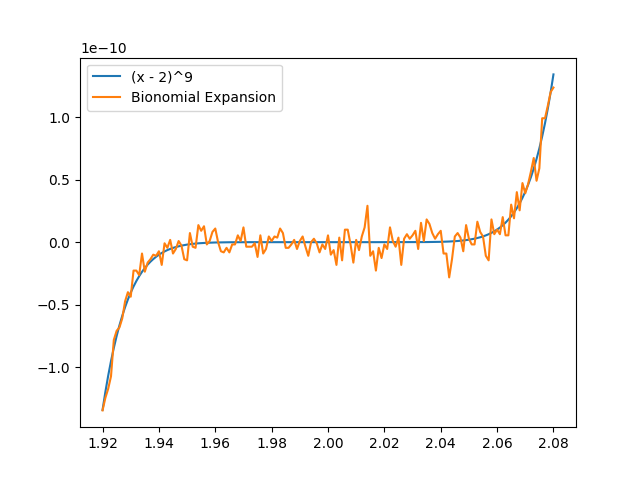
\includegraphics[width=\linewidth]{Images/problem2.png}
    \captionof{figure}{$(x - 2)^9$ versus its Bionomial Expansion}
    \label{fig:prob2}
\end{center}

It is evident that the expanded expression has a significant amount of noise. This can be attributed to
the fact that the expanded expression evaluates the summation of an alternating sequence of terms,
which are large in magnitude relative to the value of their summation. This results in a loss of precision.

For example, $2016 * 2^5 = 64512$
so that machine precision limits the absolute precision of the floating point representation of this term to about
$a_5 x^5 \epsilon \approx 64512 \cdot 10^-16 = 6.4512 \cdot 10^{-11}$ Since the summation of the sequence has a similar
order of magnitude, we see the added noise significantly affects the relative error of the function evaluations on this interval.

\section{Problem 3}
\begin{letterenum}
\item Since the absolute error $\Delta y$ is equal to $\Delta y = \Delta x_1 - \Delta x_2$,
we have absolute error:
\begin{equation*}
    |\Delta y| \leq |\Delta x_1| + |\Delta x_2|
\end{equation*}
and relative error:
\begin{equation*}
    \frac{|\Delta y|}{|y|} = \frac{|\Delta x_1| + |\Delta x_2|}{|x_1 - x_2|}
\end{equation*}
So the relative error becomes large when the true values $x_1$ and $x_2$ are
close to each other.

\item (Not sure how to manipulate this to remove the subtraction without Taylor Series...
Trigonometric sum identities don't seem to help.)

\item We compare the Taylor expansion
$z_1(\delta) = -\sin(y) \delta - 1/2 \cos(y) \delta^2$ with the floating point subtraction
expression $z_2(\delta) = \cos(y + \delta) - \cos(y)$ and evaluate at $y=1$. A plot
of $\delta$ versus $|z_1 - z_2|$ is shown in Figure (\ref{fig:prob3}).

\begin{center}
    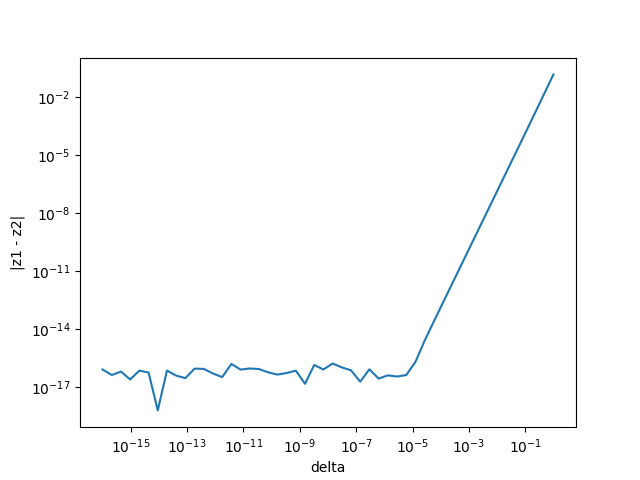
\includegraphics[width=\linewidth]{Images/problem3.png}
    \captionof{figure}{Difference between methods for evaluating $\cos(y+\delta) - \cos(y)$ at $y=1$}
    \label{fig:prob3}
\end{center}

Since the error in the Taylor series is $\mathcal{O}(\delta^3)$, we expect on a
plot with logarithmic axes that the error in the Taylor series will have a slope
of 3. For roughly $\delta > 10^{-5}$ this is indeed the case. Therefore, the direct
evaluation method is better for larger values of $\delta$.

For smaller values of $\delta$ (roughly, $\delta < 10^{-5}$) the difference is noisy and takes values
near machine precision. This suggests that the approximation with the Taylor series
is more accurate, since evaluating the floating point subtraction suffers from
rounding error.


\end{letterenum}

\section{Problem 4}

The Taylor Series of $f(x) = (1+x)^n$ at $x=0$ is given by:
\begin{equation*}
    f(x)=f(0) + f'(0) x + E(x)
\end{equation*}
where $E(x) = 1/2 f''(\zeta) x^2$ for some $\zeta$ in the interval $(0, x)$.

Since $f(0) = 1$ and $f'(0) = n ( 1+x)\eval_{x=0} = n$, it remains to show that
$E(x) = \mathcal{o}(x)$. To do so, we must show that the limit of $E(x) / x$ is 0 as
x approaches 0:
\begin{equation*}
    \lim_{x\to 0} \frac{1/2 f''(\zeta) x^2}{x}
        = \lim_{x\to 0} 1/2 f''(\zeta) x = 0
\end{equation*}


\section{Problem 5}
We must show that $x\sin(\sqrt{x}) / x^{3/2}$ is bounded by a constant in the limit
that $x$ approaches 0. Canceling terms and then using L'Hopital's Rule, we have
\begin{align*}
    \lim_{x\to 0} \frac{x \sin(\sqrt{x})}{x^{3/2}}
        = \lim_{x\to 0} \frac{ \sin(\sqrt{x})}{x^{1/2}}
        = \lim_{x\to 0} \frac{1/2 x^{-1/2} \cos(\sqrt{x})}{1/2 x^{-1/2}}
        = \lim_{x\to 0} \cos{\sqrt{x}} = 1
\end{align*}

Thus, $x \sin(\sqrt{x}) = \mathcal{O}(x^{3/2})$.







\end{letterenum}

\section{Appendix: Code}

\lstset{language=Python}
\begin{python}
import matplotlib.pyplot as plt
import numpy as np


def problem1():

    for dtype in [np.float32, np.float64]:
        eps = np.finfo(dtype).eps
        x = np.logspace(-30, 1, dtype=dtype)
        y = func1(x)
        line = plt.loglog(x, y, label=f"dtype={dtype}")[0]
        plt.axvline(x=eps, label=f"EPS({dtype})", c=line.get_color())
    plt.legend()
    plt.show()

def func1(x):
    eps = np.finfo(x.dtype).eps

    y1 = np.sqrt(x + 1) - 1
    y2 = 1/2 * x - 1/8 * x ** 2
    return np.where(x > eps, y1, y2)


#         9    8    7     6     5      4     3      2     1     0
p_coef = [1, -18, 144, -672, 2016, -4032, 5376, -4608, 2304, -512]
DEG = len(p_coef) - 1


def print_max_term():
    y = np.abs([a * 2 ** ( DEG - k) for k, a in enumerate(p_coef)])
    k = np.argmax(y)
    print(f"Max term: {p_coef[k]} * 2^{DEG - k} = {y[k]}")  # noqa

def problem2():
    p1 = lambda x: (x - 2)**9  # noqa
    p2 = lambda x:  np.sum([a * x**(DEG-k) for k, a in enumerate(p_coef)], axis=0) # noqa

    x = np.arange(1.92, 2.08, 0.001)
    y1 = p1(x)
    y2 = p2(x)
    print_max_term()

    fig = plt.figure()
    plt.plot(x, y1, label="(x - 2)^9")
    plt.plot(x, y2, label="Bionomial Expansion")
    plt.legend()
    fig.savefig("tex/hw1/Images/problem2.png")
    plt.show()



def problem3():
    y = 0
    delta = np.logspace(-16,0)
    z1 = np.cos(y + delta) - np.cos(y)
    z2 = -delta * np.sin(y) - 1/2 * delta**2 * np.cos(y)

    # fig = plt.figure()
    plt.loglog(delta, np.abs(z2-z1))
    plt.xlabel("delta")
    plt.ylabel("|z1 - z2|")
    # fig.savefig("tex/hw1/Images/problem3.png")
    plt.show()





def main():
    problem3()

if __name__ == "__main__":
    main()



\end{python}


\end{document}
